We begin by quantifying the base error inherent in the ground‑truth masks.
We then compare the segmentation performance of our two architectures.
Next, we evaluate the resulting orientation accuracy.
Finally, we examine the relationship between segmentation quality and orientation error.
All quantitative results are summarized in \cref{tab:segmentation_results,tab:orientation_results}, while key qualitative examples are shown in \cref{fig:segmentation_predictions,fig:failure_modes}.

\subsection{Dataset \& Baseline Error}
\label{subsec:baseline-error}
To quantify the inherent noise in the annotations, we compared the ground truth angles obtained from the annotations with those derived from the ground truth segmentation masks (see \Cref{tab:gt_baseline_error}).
The small discrepancy (mean $\approx$\qty{0.25}{\degree}) arises from the discretisation of the ellipses into pixelated masks, and it represents the lower bound of the achievable orientation error.
\Cref{fig:gt-baseline-error} shows the histogram and cumulative distribution function (CDF) of this baseline error.

\begin{table}[htbp]
    \centering
    \caption{Orientation error between GT masks and GT CSV angles (baseline error).}
    \label{tab:gt_baseline_error}
    \begin{tabular}{lcc}
        \toprule
        \textbf{Metric}    & \textbf{Error}      \\
        \midrule
        Mean               & \qty{0.25}{\degree} \\
        Std. Dev.          & \qty{0.20}{\degree} \\
        Median             & \qty{0.22}{\degree} \\
        \midrule
        Percentiles        &                     \\
        \qty{50}{\percent} & \qty{0.22}{\degree} \\
        \qty{75}{\percent} & \qty{0.39}{\degree} \\
        \qty{90}{\percent} & \qty{0.54}{\degree} \\
        \qty{95}{\percent} & \qty{0.62}{\degree} \\
        \qty{99}{\percent} & \qty{0.74}{\degree} \\
        Max                & \qty{0.85}{\degree} \\
        \bottomrule
    \end{tabular}
\end{table}


\subsection{Segmentation Performance}
\label{subsec:segmentation-performance}
First, we evaluate the segmentation quality of both models on the test set, reporting per‑class IoU and foreground mIoU over the head and tail classes.

\Cref{tab:segmentation_results} summarizes the results: ResUNet18 substantially outperforms UNet3 across all classes, achieving a foreground mIoU of \qty{0.71}{} compared to \qty{0.48}{} for UNet3.
ResUNet18 also achieves a notably lower segmentation loss and a higher background IoU.

\Cref{fig:segmentation_loss_curves} shows the training and validation loss curves over 10 epochs.
Both models converge quickly, but ResUNet18 starts to overfit after around four epochs, as indicated by an increase in validation loss.
Nevertheless, ResUNet18 consistently achieves lower losses than UNet3 throughout training -- UNet3 never reaches ResUNet18's loss levels, even at its best.

\Cref{fig:segmentation_predictions} presents qualitative predictions for three test samples for each model.
Each example shows the input image, the ground-truth mask and the predicted mask.
ResUNet18's predictions appear sharper and more accurate, with clear distinction between the head and tail, whereas UNet3's predictions are blurrier and more easily confused by noise from other bees or background clutter.

\begin{table}[htbp]
    \centering
    \caption{Segmentation performance on the test set.}
    \label{tab:segmentation_results}
    \begin{tabular}{lcccccc}
        \toprule
        \textbf{Model} & \textbf{\#Params} & \textbf{Test Loss} & \textbf{IoU$_{0}$} & \textbf{IoU$_{1}$} & \textbf{IoU$_{2}$} & \textbf{mIoU$_{1,2}$} \\
        \midrule
        UNet3          & \qty{1.93}{M}     & \qty{0.3620}{}     & \qty{0.8959}{}     & \qty{0.4852}{}     & \qty{0.4827}{}     & \qty{0.4839}{}        \\
        ResUNet18      & \qty{14.24}{M}    & \qty{0.1742}{}     & \qty{0.9482}{}     & \qty{0.7069}{}     & \qty{0.7205}{}    & \qty{0.7137}{}       \\
        \bottomrule
    \end{tabular}
\end{table}

\begin{figure}[htbp]
    \centering
    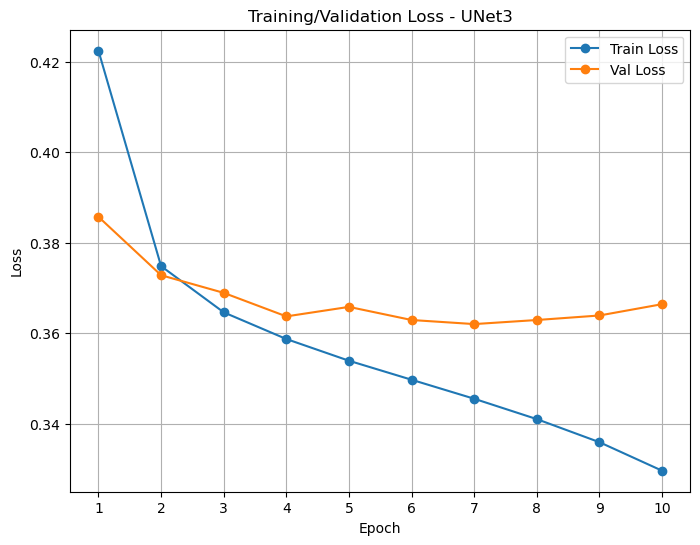
\includegraphics[width=0.49\textwidth]{figures/results/2 - segmentation performance/UNet3 Loss.png}
    \hfill
    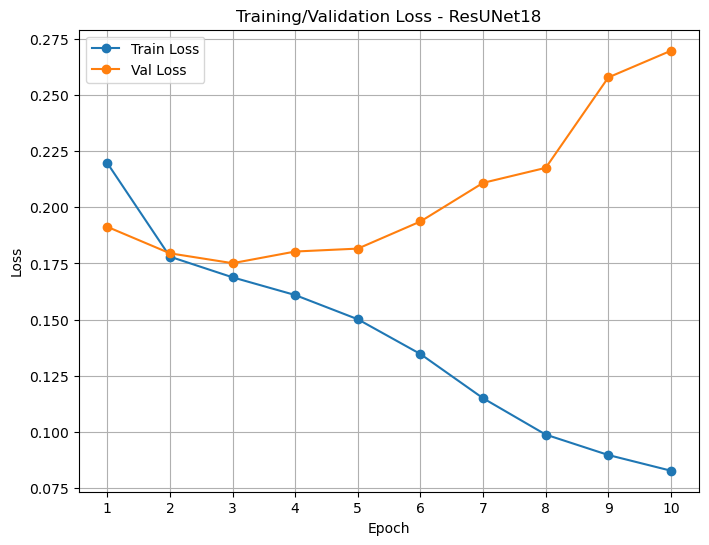
\includegraphics[width=0.49\textwidth]{figures/results/2 - segmentation performance/ResUNet18 Loss.png}
    \caption{
        Training and validation loss curves over 10 epochs for both models.
        (\textbf{Left}) UNet3 shows steady convergence but plateaus at a higher loss.
        (\textbf{Right}) ResUNet18 achieves lower training and validation loss overall but begins to overfit after about 4 epochs, as indicated by the upward trend in validation loss.
    }
    \label{fig:segmentation_loss_curves}
\end{figure}

\begin{figure}[htbp]
    \centering
    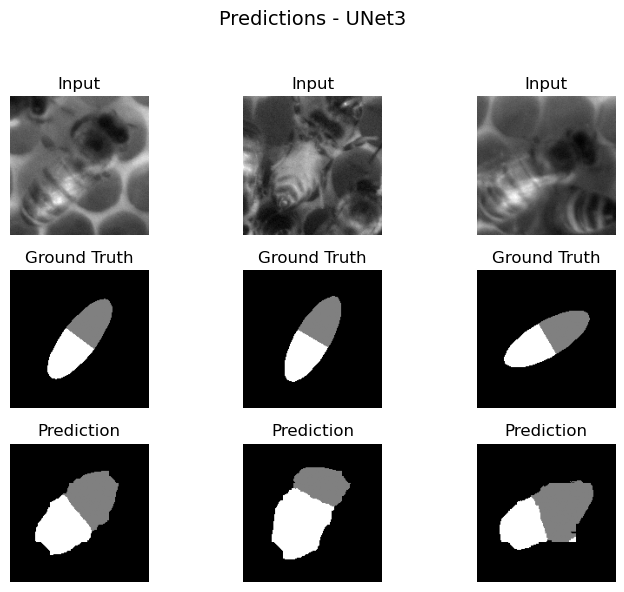
\includegraphics[width=0.49\textwidth]{figures/results/2 - segmentation performance/UNet3 Prediction Masks.png}
    \hfill
    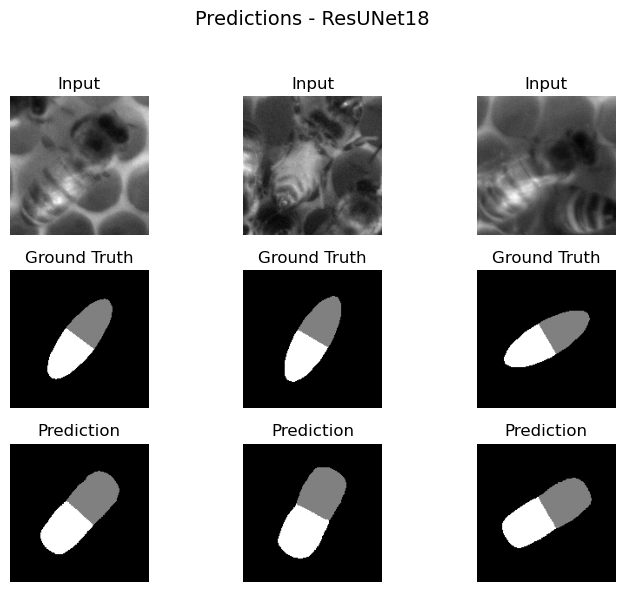
\includegraphics[width=0.49\textwidth]{figures/results/2 - segmentation performance/ResUNet18 Prediction Masks.png}
    \caption{
        Example segmentation predictions on three test samples for each model.
        Each column shows (\textit{top}) the input image, (\textit{middle}) the ground‑truth mask, and (\textit{bottom}) the predicted mask.
        (\textbf{Left}) UNet3 predictions are blurry and frequently misclassify head/tail regions due to noise and clutter.
        (\textbf{Right}) ResUNet18 predictions are sharper and better capture head and tail shapes, even in the presence of background bees and occlusions.
    }
    \label{fig:segmentation_predictions}
\end{figure}

\subsection{Orientation Estimation}
\label{subsec:orientation-estimation}
Next, we evaluate the models’ ability to predict the bees’ orientation angles based on the predicted head and tail masks.
\Cref{tab:orientation_results} summarizes the orientation error on the test set, reported as the mean, median and key percentiles.

ResUNet18 achieves slightly better orientation accuracy than UNet3: the mean error is reduced from \qty{14.8}{\degree} to \qty{13.2}{\degree}, and the median error from \qty{6.5}{\degree} to \qty{5.7}{\degree}.
However, both models remain well above the baseline error of approximately \qty{0.25}{\degree} measured between the ground-truth masks and the ground-truth CSV angles.
This suggests that imperfect segmentations rather than annotation noise are the main limiting factor.

\Cref{fig:orientation_error_hist_cdf} shows the distribution of absolute orientation errors for each model, presented as both a histogram and a CDF.
Both models exhibit a strong concentration of predictions with errors below \qty{20}{\degree}, with ResUNet18 producing slightly more low-error predictions than UNet3.
The overall distributions are otherwise similar, with both models displaying a noticeable secondary peak at very high errors (approximately \qty{180}{\degree}), which is likely caused by head–tail confusion or annotation errors.
We investigate this phenomenon further in \cref{subsec:qualitative-analysis}.

We also examined the signed orientation errors to check for systematic directional bias in the predictions (see \Cref{fig:appendix_unet3_orientation,fig:appendix_resunet18_orientation}).
No substantial bias was observed, with the errors being approximately symmetrically distributed around zero.


\begin{table}[htbp]
    \centering
    \caption{Absolute orientation error against ground‑truth CSV angles.}
    \label{tab:orientation_results}
    \begin{tabular}{lcccccc}
        \toprule
        \textbf{Model} & \textbf{Mean $\pm$ SD}                          & \textbf{Median}     & \textbf{75\%ile}     & \textbf{90\%ile} & \textbf{95\%ile} & \textbf{99\%ile} \\
        \midrule
        UNet3          & \qty{14.79}{\degree} $\pm$ \qty{31.57}{\degree} & \qty{6.49}{\degree} & \qty{12.16}{\degree}   & \qty{21.91}{\degree}   & \qty{50.57}{\degree}   & \qty{174.60}{\degree}  \\
        ResUNet18      & \qty{13.23}{\degree} $\pm$ \qty{31.12}{\degree} & \qty{5.73}{\degree} & \qty{10.59}{\degree}   & \qty{17.98}{\degree}   & \qty{30.25}{\degree}   & \qty{175.74}{\degree}  \\
        \bottomrule
    \end{tabular}
\end{table}

\begin{figure}[htbp]
    \centering
    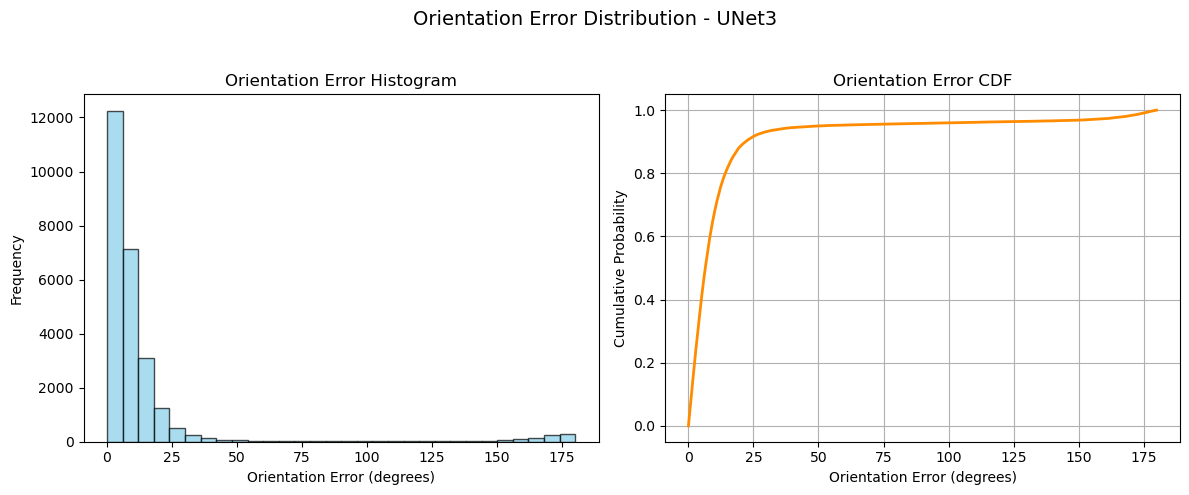
\includegraphics[width=\textwidth]{figures/results/3 - orientation estimation/UNet3 Orientation Error.png}

    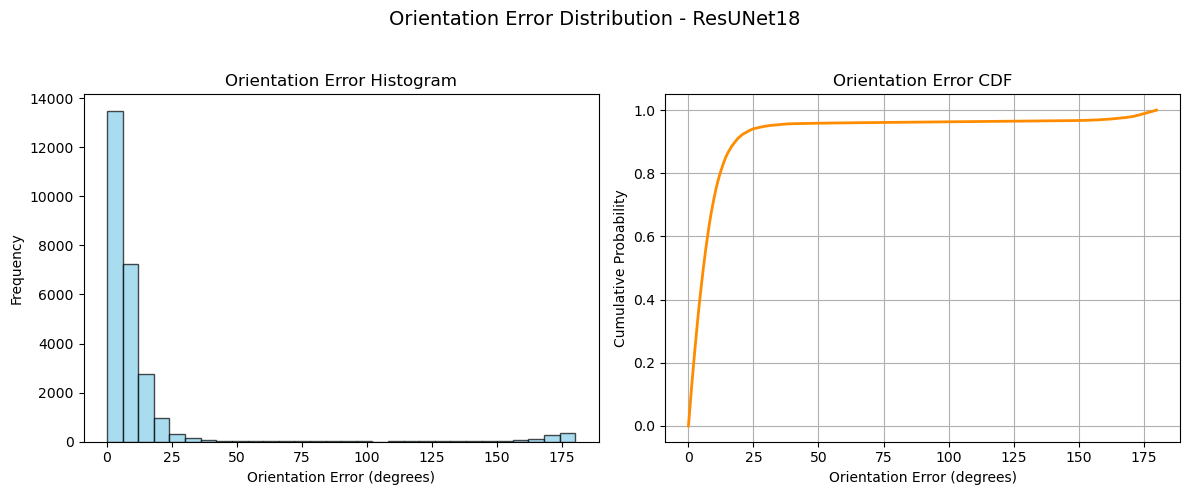
\includegraphics[width=\textwidth]{figures/results/3 - orientation estimation/ResUNet18 Orientation Error.png}
    \caption{
        Orientation error distribution on the test set for UNet3 (\textbf{top}) and ResUNet18 (\textbf{bottom}).
        For each model, the left panel shows a histogram of absolute orientation errors; the right panel shows the cumulative distribution function (CDF).
        Both models produce similar distributions with most errors below \qty{20}{\degree} and a small bump at very high errors ($\approx$\qty{180}{\degree}).
    }
    \label{fig:orientation_error_hist_cdf}
\end{figure}

\subsection{IoU vs. Orientation Error Relationship}
\label{subsec:correlation}
We next investigate the relationship between segmentation quality and orientation accuracy.
Specifically, we analyze whether higher foreground mIoU correlates with lower orientation errors.

\Cref{fig:iou_vs_orientation_error} shows hexbin plots of foreground mIoU versus absolute orientation error for UNet3 and ResUNet18 on the test set.
A clear negative correlation is evident for both models, as confirmed by Spearman's rank correlation ($\rho = -0.40$, $p < 0.001$ for UNet3 and $-0.73$, $p < 0.001$ for ResUNet18)~\cite{noauthor_nodate_spearmans}: as mIoU increases, orientation error decreases.

However, ResUNet18 predictions are concentrated more tightly in the top left of the plot (high mIoU and low error), while UNet3 predictions are more scattered.
UNet3 produces many examples with low mIoU even when the orientation error is moderate ($\leq$\qty{50}{\degree}), whereas ResUNet18’s predictions are more consistent, with higher mIoU and less variation.

This suggests that better segmentation masks (higher mIoU) generally enable more accurate orientation estimation and that ResUNet18 produces more consistent and reliable segmentations.

We also examined the signed orientation error as a function of the ground-truth angle (see \Cref{fig:appendix_unet3_orientation,fig:appendix_resunet18_orientation}).
No clear dependency was observed; the error distribution appears uniform across the range of ground-truth angles.


\begin{figure}[htbp]
    \centering
    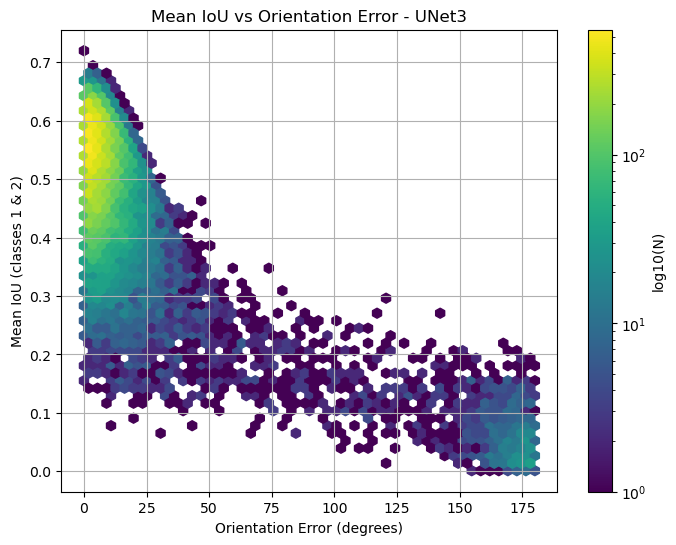
\includegraphics[width=0.49\textwidth]{figures/results/4 - correlation/UNet3 mIoU vs Orientation Error.png}
    \hfill
    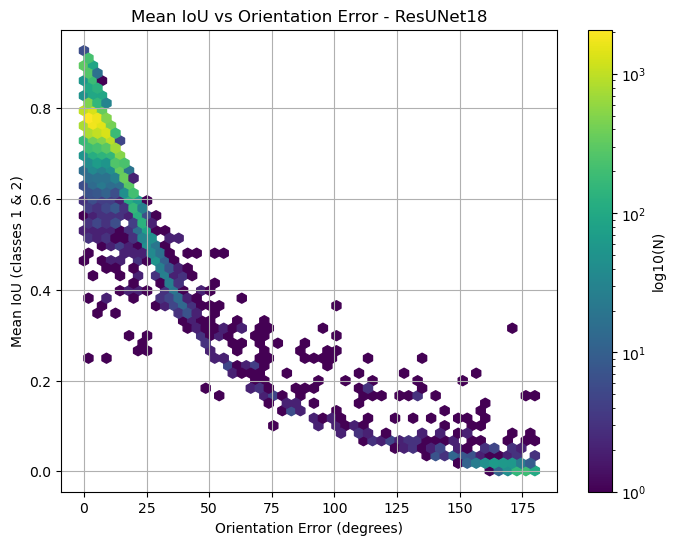
\includegraphics[width=0.49\textwidth]{figures/results/4 - correlation/ResUNet18 mIoU vs Orientation Error.png}
    \caption{
        Hexbin plots of foreground mIoU versus absolute orientation error for (\textbf{left}) UNet3 and (\textbf{right}) ResUNet18.
        Both models exhibit a negative correlation (Spearman’s $\rho = -0.40$ for UNet3, $\rho = -0.73$ for ResUNet18), but ResUNet18 predictions are more concentrated in the upper‑left corner (high mIoU, low error).
        In contrast, UNet3 predictions are dispersed with a broader spread of mIoU for any error.
    }
    \label{fig:iou_vs_orientation_error}
\end{figure}

\subsection{Qualitative Analysis}
\label{subsec:qualitative-analysis}
To gain a better understanding of the areas in which the models are struggling, we conducted a qualitative analysis of failure cases from the test set.
We focused on examples with significant orientation errors, particularly those around \qty{90}{\degree} and \qty{180}{\degree}, as these are indicative of challenging scenarios or annotation issues.

Representative examples are shown in the appendix (\Cref{fig:failure_modes}), grouped by error type. Each panel displays the input image, the ground-truth mask, the predicted mask, and the measured orientation error.

For \qty{180}{\degree} errors, the majority appear to stem from annotation errors rather than model mistakes: in all the examples shown, the annotated head and tail regions are reversed compared to the visible anatomy, while the model predictions point in the correct direction despite the imperfect masks.
For instance, the UNet3 prediction in the first image provides a blurry yet correctly oriented segmentation, whereas the annotation erroneously labels the tail as the head.
Similarly, the ResUNet18 predictions align well with the actual bee orientation, even when the annotation is flipped.

Both models struggle with \qty{90}{\degree} errors in highly cluttered images where no bee is fully visible.
In the UNet3 examples, the predicted masks are diffuse and are often confused by surrounding bees.
The annotations themselves are ambiguous or clearly do not correspond to any individual bee.
ResUNet18 performs better, often correctly segmenting one plausible bee even when the annotation does not correspond to it.
In some cases, the image quality or visibility is so poor that neither the model nor the annotation appears reliable.

These examples highlight the limitations of the models, particularly in cluttered and low-quality regions, as well as the inconsistencies in the ground-truth annotations, which may artificially inflate measured errors.
